\documentclass[a4paper,11pt]{article}
\usepackage{graphicx}
\usepackage{pifont}
\usepackage{ulem}
\usepackage{supertabular}
\usepackage{fancyhdr}
\usepackage{rotating}
\usepackage{verbatim}
\usepackage{appendix}

\voffset -1.5cm
\hoffset 0.0cm
\textheight 25cm
\textwidth 16cm
\topmargin 0.0cm
\oddsidemargin 0.0cm
\evensidemargin 0.0cm

\newcommand{\VROT}[1]{\begin{turn}{90}#1\end{turn}}     % vertical text
\def\X{$\surd$}     % tick symbol

\newenvironment{script}{\endgraf\footnotesize\verbatim}{\endverbatim}

\usepackage{hyperref}%                   % Utilisation de HyperTeX

\hypersetup{
    pdfauthor   = {Daniel Gracia P\'erez},%
    pdftitle    = {UNISIM ARMEmu Simulator Manual},%
    pdfsubject  = {UNISIM},%
    pdfkeywords = {simulation framework, architectural exploration, embedded system design, system verification},%
    pdfcreator  = {rubber},%
    pdfproducer = {rubber}
}

\begin{document}
% \addtolength{\hoffset}{-2.0cm}
% \addtolength{\voffset}{-2.0cm}
\title{UNISIM\\ ARMEmu Simulator Manual}
\author{Daniel Gracia P\'erez}
\date{}

\maketitle
\tableofcontents
\listoffigures
\listoftables

\newpage
\section{Simulator technical reference (generated)}
This documentation has been automatically generated from the simulator \texttt{UNISIM ARMEmu} version 0.7.1 on Jun 26 2013.
\subsection{Introduction}
UNISIM ARMv5 User Level Simulator.\\
Section \ref{UNISIM ARMEmu_licensing} gives licensing informations about the simulator.
Section \ref{UNISIM ARMEmu_simulated_configuration} shows the set of modules and services that compose the simulator.
Section \ref{UNISIM ARMEmu_using} shows how to invoke the simulator at the command line prompt.
Section \ref{UNISIM ARMEmu_configuration} gives the simulator parameters.
Section \ref{UNISIM ARMEmu_statistics} gives the simulator statistic counters.
Section \ref{UNISIM ARMEmu_formulas} gives the simulator statistic formulas.
\subsection{Licensing}
\label{UNISIM ARMEmu_licensing}
UNISIM ARMEmu 0.7.1\\
Copyright (C) 2007-2010, Commissariat a l'Energie Atomique\\
License: BSD (See file COPYING)\\
Authors: Daniel Gracia Perez (daniel.gracia-perez@cea.fr)\\
\subsection{Simulated configuration}
\label{UNISIM ARMEmu_simulated_configuration}
\begin{figure}[!ht]
	\begin{center}
		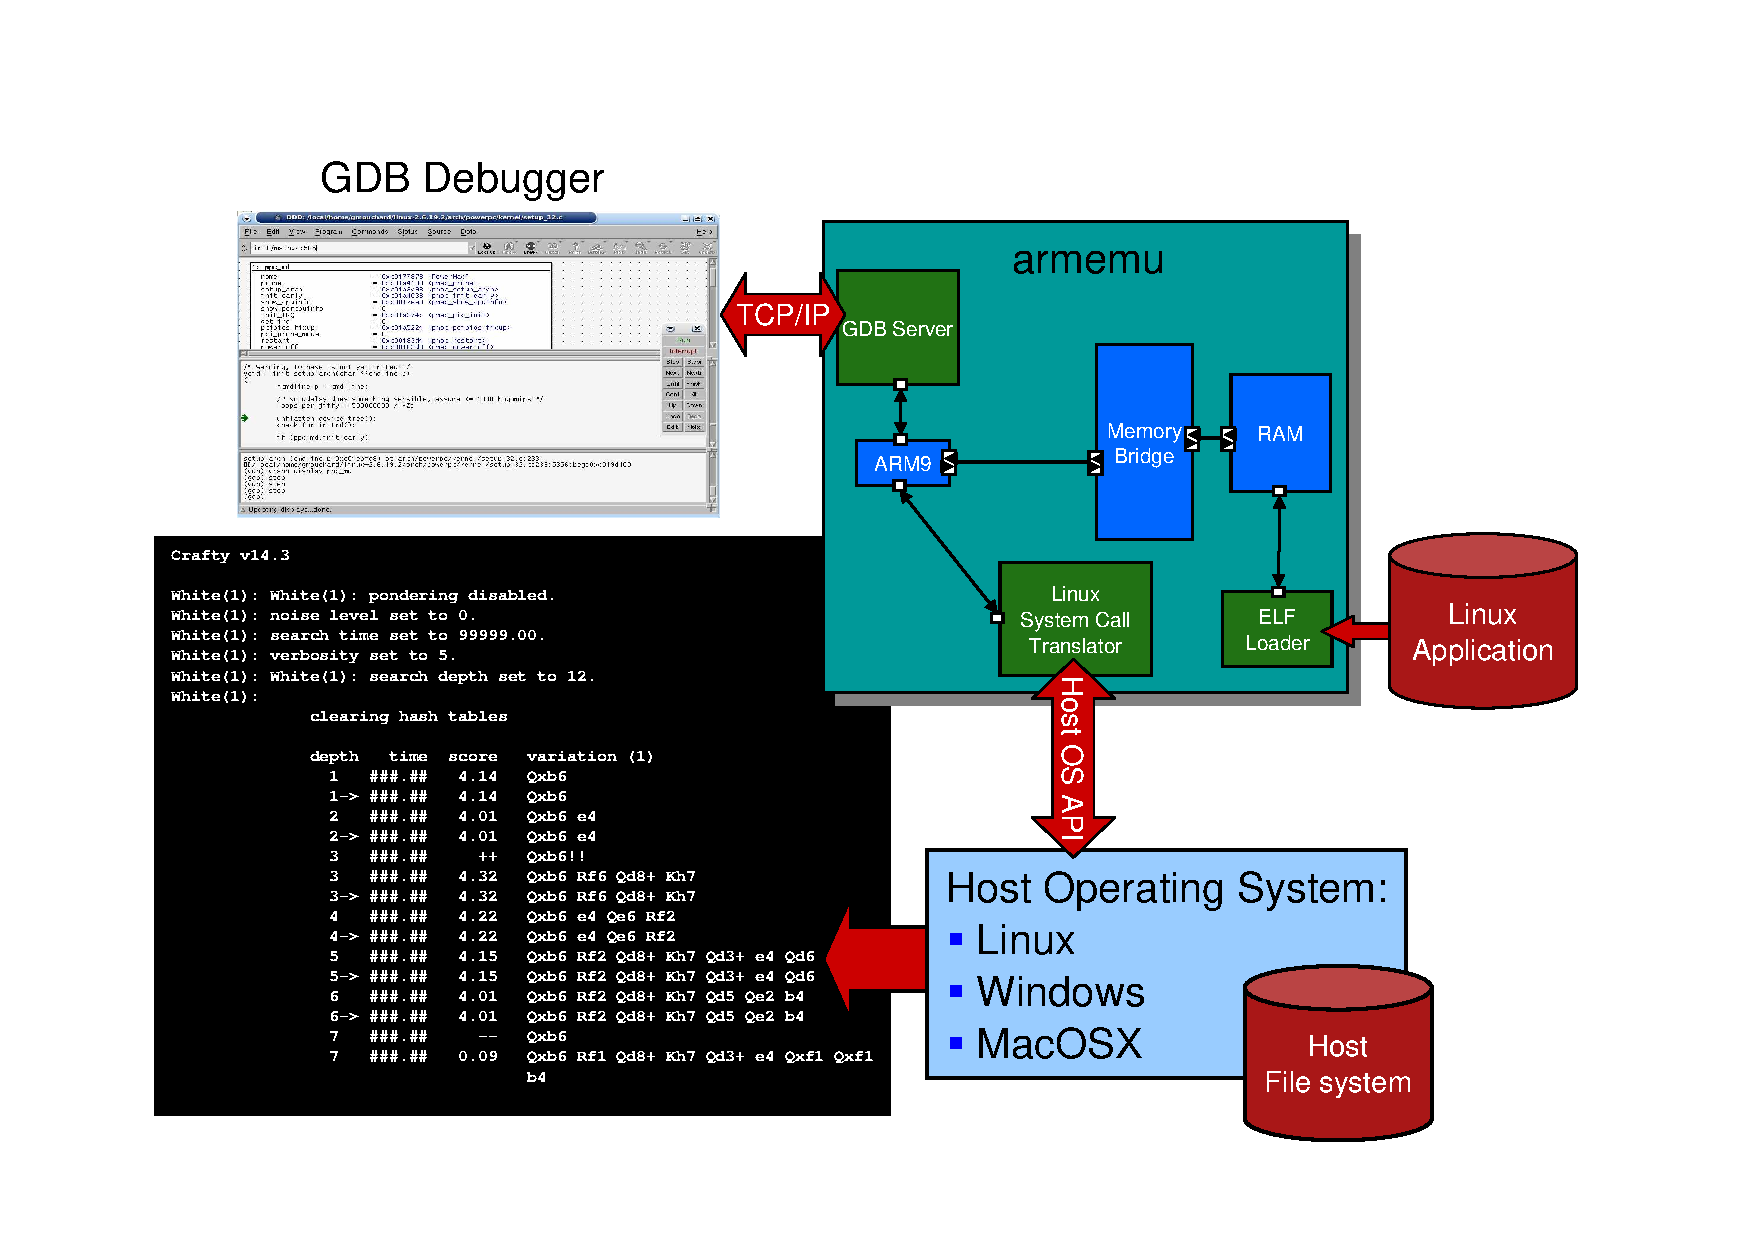
\includegraphics[width=\textwidth]{armemu/fig_schematic.pdf}
	\end{center}
	\caption{UNISIM ARMEmu simulator schematic.}
\end{figure}
\noindent The UNISIM ARMEmu simulator is composed of the following modules and services:
\begin{itemize}\addtolength{\itemsep}{-0.40\baselineskip}
\item \textbf{cpu}
\item \textbf{cpu.dcache}
\item \textbf{cpu.icache}
\item \textbf{debugger}
\item \textbf{gdb-server}: this service implements the GDB server remote serial protocol over TCP/IP. Standards GDB clients (e.g. gdb, eclipse, ddd) can connect to the simulator to debug the target application that runs within the simulator.
\item \textbf{host-time}: this service is an abstraction layer for the host machine time
\item \textbf{inline-debugger}: this service implements a built-in debugger in the terminal console
\item \textbf{linux-os}
\item \textbf{memory}: this module implements a memory
\item \textbf{profiler}
\item \textbf{tee-memory-access-reporting}
\item \textbf{tee-memory-access-reporting.tee-memory-access-reporting.control\_selector[0]}
\item \textbf{tee-memory-access-reporting.tee-memory-access-reporting.control\_selector[10]}
\item \textbf{tee-memory-access-reporting.tee-memory-access-reporting.control\_selector[11]}
\item \textbf{tee-memory-access-reporting.tee-memory-access-reporting.control\_selector[12]}
\item \textbf{tee-memory-access-reporting.tee-memory-access-reporting.control\_selector[13]}
\item \textbf{tee-memory-access-reporting.tee-memory-access-reporting.control\_selector[14]}
\item \textbf{tee-memory-access-reporting.tee-memory-access-reporting.control\_selector[15]}
\item \textbf{tee-memory-access-reporting.tee-memory-access-reporting.control\_selector[1]}
\item \textbf{tee-memory-access-reporting.tee-memory-access-reporting.control\_selector[2]}
\item \textbf{tee-memory-access-reporting.tee-memory-access-reporting.control\_selector[3]}
\item \textbf{tee-memory-access-reporting.tee-memory-access-reporting.control\_selector[4]}
\item \textbf{tee-memory-access-reporting.tee-memory-access-reporting.control\_selector[5]}
\item \textbf{tee-memory-access-reporting.tee-memory-access-reporting.control\_selector[6]}
\item \textbf{tee-memory-access-reporting.tee-memory-access-reporting.control\_selector[7]}
\item \textbf{tee-memory-access-reporting.tee-memory-access-reporting.control\_selector[8]}
\item \textbf{tee-memory-access-reporting.tee-memory-access-reporting.control\_selector[9]}
\item \textbf{time}: this service is an abstraction layer for the SystemC kernel time
\end{itemize}
\subsection{Using the UNISIM ARMEmu simulator}
\label{UNISIM ARMEmu_using}
The UNISIM ARMEmu simulator has the following command line options:\\
~\\
\noindent Usage: \texttt{unisim-armemu-0.7.1 [<options>] [...]}

\noindent Options:
\begin{itemize}
\item \texttt{--set $<$param=value$>$ or -s $<$param=value$>$}: set value of parameter 'param' to 'value'
\item \texttt{--config $<$XML file$>$ or -c $<$XML file$>$}: configures the simulator with the given XML configuration file
\item \texttt{--get-config $<$XML file$>$ or -g $<$XML file$>$}: get the simulator configuration XML file (you can use it to create your own configuration. This option can be combined with -c to get a new configuration file with existing variables from another file
\item \texttt{--list or -l}: lists all available parameters, their type, and their current value
\item \texttt{--warn or -w}: enable printing of kernel warnings
\item \texttt{--doc $<$Latex file$>$ or -d $<$Latex file$>$}: enable printing a latex documentation
\item \texttt{--version or -v}: displays the program version information
\item \texttt{--share-path $<$path$>$ or -p $<$path$>$}: the path that should be used for the share directory (absolute path)
\item \texttt{--help or -h}: displays this help
\end{itemize}
\subsection{Configuration}
\label{UNISIM ARMEmu_configuration}
Simulator configuration (see below) can be modified using command line Options \texttt{--set $<$param=value$>$} or \texttt{--config $<$config file$>$}.\\
~\\
\tablehead{\hline}
\tabletail{\hline}
\begin{supertabular}{|p{7.5cm}|p{7.5cm}|}
\multicolumn{2}{|l|}{\textbf{\Large Global}}\\
\hline
\multicolumn{1}{|p{7.5cm}}{\textbf{Name:} \texttt{enable-gdb-server}} & \multicolumn{1}{p{7.5cm}|}{\textbf{Type:} \texttt{parameter}}\\
\multicolumn{1}{|p{7.5cm}}{\textbf{Default:} \texttt{true}} & \multicolumn{1}{p{7.5cm}|}{\textbf{Data type:} \texttt{boolean}}\\
\multicolumn{2}{|p{15cm}|}{\textbf{Valid:} \texttt{true},~\texttt{false}}\\
\multicolumn{2}{|l|}{}\\
\multicolumn{2}{|p{15cm}|}{\textbf{Description:} \newline Enable GDB server..}\\
\hline
\multicolumn{1}{|p{7.5cm}}{\textbf{Name:} \texttt{enable-inline-debugger}} & \multicolumn{1}{p{7.5cm}|}{\textbf{Type:} \texttt{parameter}}\\
\multicolumn{1}{|p{7.5cm}}{\textbf{Default:} \texttt{true}} & \multicolumn{1}{p{7.5cm}|}{\textbf{Data type:} \texttt{boolean}}\\
\multicolumn{2}{|p{15cm}|}{\textbf{Valid:} \texttt{true},~\texttt{false}}\\
\multicolumn{2}{|l|}{}\\
\multicolumn{2}{|p{15cm}|}{\textbf{Description:} \newline Enable inline debugger..}\\
\hline
\multicolumn{1}{|p{7.5cm}}{\textbf{Name:} \texttt{enable-power-estimation}} & \multicolumn{1}{p{7.5cm}|}{\textbf{Type:} \texttt{parameter}}\\
\multicolumn{1}{|p{7.5cm}}{\textbf{Default:} \texttt{false}} & \multicolumn{1}{p{7.5cm}|}{\textbf{Data type:} \texttt{boolean}}\\
\multicolumn{2}{|p{15cm}|}{\textbf{Valid:} \texttt{true},~\texttt{false}}\\
\multicolumn{2}{|l|}{}\\
\multicolumn{2}{|p{15cm}|}{\textbf{Description:} \newline Activate caches power estimation..}\\
\hline
\multicolumn{1}{|p{7.5cm}}{\textbf{Name:} \texttt{enable-press-enter-at-exit}} & \multicolumn{1}{p{7.5cm}|}{\textbf{Type:} \texttt{parameter}}\\
\multicolumn{1}{|p{7.5cm}}{\textbf{Default:} \texttt{false}} & \multicolumn{1}{p{7.5cm}|}{\textbf{Data type:} \texttt{boolean}}\\
\multicolumn{2}{|p{15cm}|}{\textbf{Valid:} \texttt{true},~\texttt{false}}\\
\multicolumn{2}{|l|}{}\\
\multicolumn{2}{|p{15cm}|}{\textbf{Description:} \newline Enable/Disable pressing key enter at exit.}\\
\hline
\multicolumn{1}{|p{7.5cm}}{\textbf{Name:} \texttt{kernel\_logger.file}} & \multicolumn{1}{p{7.5cm}|}{\textbf{Type:} \texttt{parameter}}\\
\multicolumn{1}{|p{7.5cm}}{\textbf{Default:} \texttt{false}} & \multicolumn{1}{p{7.5cm}|}{\textbf{Data type:} \texttt{boolean}}\\
\multicolumn{2}{|p{15cm}|}{\textbf{Valid:} \texttt{true},~\texttt{false}}\\
\multicolumn{2}{|l|}{}\\
\multicolumn{2}{|p{15cm}|}{\textbf{Description:} \newline Keep logger output in a file.}\\
\hline
\multicolumn{1}{|p{7.5cm}}{\textbf{Name:} \texttt{kernel\_logger.filename}} & \multicolumn{1}{p{7.5cm}|}{\textbf{Type:} \texttt{parameter}}\\
\multicolumn{1}{|p{7.5cm}}{\textbf{Default:} \texttt{logger\_output.txt}} & \multicolumn{1}{p{7.5cm}|}{\textbf{Data type:} \texttt{string}}\\
\multicolumn{2}{|l|}{}\\
\multicolumn{2}{|l|}{}\\
\multicolumn{2}{|p{15cm}|}{\textbf{Description:} \newline Filename to keep logger output \_(the option file must be activated).}\\
\hline
\multicolumn{1}{|p{7.5cm}}{\textbf{Name:} \texttt{kernel\_logger.std\_err}} & \multicolumn{1}{p{7.5cm}|}{\textbf{Type:} \texttt{parameter}}\\
\multicolumn{1}{|p{7.5cm}}{\textbf{Default:} \texttt{true}} & \multicolumn{1}{p{7.5cm}|}{\textbf{Data type:} \texttt{boolean}}\\
\multicolumn{2}{|p{15cm}|}{\textbf{Valid:} \texttt{true},~\texttt{false}}\\
\multicolumn{2}{|l|}{}\\
\multicolumn{2}{|p{15cm}|}{\textbf{Description:} \newline Show logger output through the standard error output.}\\
\hline
\multicolumn{1}{|p{7.5cm}}{\textbf{Name:} \texttt{kernel\_logger.std\_err\_color}} & \multicolumn{1}{p{7.5cm}|}{\textbf{Type:} \texttt{parameter}}\\
\multicolumn{1}{|p{7.5cm}}{\textbf{Default:} \texttt{true}} & \multicolumn{1}{p{7.5cm}|}{\textbf{Data type:} \texttt{boolean}}\\
\multicolumn{2}{|p{15cm}|}{\textbf{Valid:} \texttt{true},~\texttt{false}}\\
\multicolumn{2}{|l|}{}\\
\multicolumn{2}{|p{15cm}|}{\textbf{Description:} \newline Colorize logger output through the standard error output \_(only works if std\_err is active).}\\
\hline
\multicolumn{1}{|p{7.5cm}}{\textbf{Name:} \texttt{kernel\_logger.std\_out}} & \multicolumn{1}{p{7.5cm}|}{\textbf{Type:} \texttt{parameter}}\\
\multicolumn{1}{|p{7.5cm}}{\textbf{Default:} \texttt{false}} & \multicolumn{1}{p{7.5cm}|}{\textbf{Data type:} \texttt{boolean}}\\
\multicolumn{2}{|p{15cm}|}{\textbf{Valid:} \texttt{true},~\texttt{false}}\\
\multicolumn{2}{|l|}{}\\
\multicolumn{2}{|p{15cm}|}{\textbf{Description:} \newline Show logger output through the standard output.}\\
\hline
\multicolumn{1}{|p{7.5cm}}{\textbf{Name:} \texttt{kernel\_logger.std\_out\_color}} & \multicolumn{1}{p{7.5cm}|}{\textbf{Type:} \texttt{parameter}}\\
\multicolumn{1}{|p{7.5cm}}{\textbf{Default:} \texttt{false}} & \multicolumn{1}{p{7.5cm}|}{\textbf{Data type:} \texttt{boolean}}\\
\multicolumn{2}{|p{15cm}|}{\textbf{Valid:} \texttt{true},~\texttt{false}}\\
\multicolumn{2}{|l|}{}\\
\multicolumn{2}{|p{15cm}|}{\textbf{Description:} \newline Colorize logger output through the standard output \_(only works if std\_out is active).}\\
\hline
\multicolumn{1}{|p{7.5cm}}{\textbf{Name:} \texttt{kernel\_logger.xml\_file}} & \multicolumn{1}{p{7.5cm}|}{\textbf{Type:} \texttt{parameter}}\\
\multicolumn{1}{|p{7.5cm}}{\textbf{Default:} \texttt{false}} & \multicolumn{1}{p{7.5cm}|}{\textbf{Data type:} \texttt{boolean}}\\
\multicolumn{2}{|p{15cm}|}{\textbf{Valid:} \texttt{true},~\texttt{false}}\\
\multicolumn{2}{|l|}{}\\
\multicolumn{2}{|p{15cm}|}{\textbf{Description:} \newline Keep logger output in a file xml formatted.}\\
\hline
\multicolumn{1}{|p{7.5cm}}{\textbf{Name:} \texttt{kernel\_logger.xml\_file\_gzipped}} & \multicolumn{1}{p{7.5cm}|}{\textbf{Type:} \texttt{parameter}}\\
\multicolumn{1}{|p{7.5cm}}{\textbf{Default:} \texttt{false}} & \multicolumn{1}{p{7.5cm}|}{\textbf{Data type:} \texttt{boolean}}\\
\multicolumn{2}{|p{15cm}|}{\textbf{Valid:} \texttt{true},~\texttt{false}}\\
\multicolumn{2}{|l|}{}\\
\multicolumn{2}{|p{15cm}|}{\textbf{Description:} \newline If the xml\_file option is active, the output file will be compressed (a .gz extension will be automatically added to the xml\_filename option.}\\
\hline
\multicolumn{1}{|p{7.5cm}}{\textbf{Name:} \texttt{kernel\_logger.xml\_filename}} & \multicolumn{1}{p{7.5cm}|}{\textbf{Type:} \texttt{parameter}}\\
\multicolumn{1}{|p{7.5cm}}{\textbf{Default:} \texttt{logger\_output.xml}} & \multicolumn{1}{p{7.5cm}|}{\textbf{Data type:} \texttt{string}}\\
\multicolumn{2}{|l|}{}\\
\multicolumn{2}{|l|}{}\\
\multicolumn{2}{|p{15cm}|}{\textbf{Description:} \newline Filename to keep logger xml output \_(the option xml\_file must be activated).}\\
\hline
\hline
\multicolumn{2}{|l|}{\textbf{\Large cpu}}\\
\hline
\multicolumn{1}{|p{7.5cm}}{\textbf{Name:} \texttt{cpu.default-endianness}} & \multicolumn{1}{p{7.5cm}|}{\textbf{Type:} \texttt{parameter}}\\
\multicolumn{1}{|p{7.5cm}}{\textbf{Default:} \texttt{little-endian}} & \multicolumn{1}{p{7.5cm}|}{\textbf{Data type:} \texttt{string}}\\
\multicolumn{2}{|l|}{}\\
\multicolumn{2}{|l|}{}\\
\multicolumn{2}{|p{15cm}|}{\textbf{Description:} \newline The processor default/boot endianness. Available values are: little-endian and big-endian..}\\
\hline
\multicolumn{1}{|p{7.5cm}}{\textbf{Name:} \texttt{cpu.voltage}} & \multicolumn{1}{p{7.5cm}|}{\textbf{Type:} \texttt{parameter}}\\
\multicolumn{1}{|p{7.5cm}}{\textbf{Default:} \texttt{1800}} & \multicolumn{1}{p{7.5cm}|}{\textbf{Data type:} \texttt{unsigned 64-bit integer}}\\
\multicolumn{2}{|l|}{}\\
\multicolumn{2}{|l|}{}\\
\multicolumn{2}{|p{15cm}|}{\textbf{Description:} \newline The processor voltage in mV..}\\
\hline
\multicolumn{1}{|p{7.5cm}}{\textbf{Name:} \texttt{cpu.verbose}} & \multicolumn{1}{p{7.5cm}|}{\textbf{Type:} \texttt{parameter}}\\
\multicolumn{1}{|p{7.5cm}}{\textbf{Default:} \texttt{0x00000000}} & \multicolumn{1}{p{7.5cm}|}{\textbf{Data type:} \texttt{unsigned 32-bit integer}}\\
\multicolumn{2}{|l|}{}\\
\multicolumn{2}{|l|}{}\\
\multicolumn{2}{|p{15cm}|}{\textbf{Description:} \newline Activate the verbose system (0 = inactive, different than 0 = active)..}\\
\hline
\multicolumn{1}{|p{7.5cm}}{\textbf{Name:} \texttt{cpu.trap-on-instruction-counter}} & \multicolumn{1}{p{7.5cm}|}{\textbf{Type:} \texttt{parameter}}\\
\multicolumn{1}{|p{7.5cm}}{\textbf{Default:} \texttt{0}} & \multicolumn{1}{p{7.5cm}|}{\textbf{Data type:} \texttt{unsigned 64-bit integer}}\\
\multicolumn{2}{|l|}{}\\
\multicolumn{2}{|l|}{}\\
\multicolumn{2}{|p{15cm}|}{\textbf{Description:} \newline Produce a trap when the given instruction count is reached..}\\
\hline
\multicolumn{1}{|p{7.5cm}}{\textbf{Name:} \texttt{cpu.cpu-cycle-time}} & \multicolumn{1}{p{7.5cm}|}{\textbf{Type:} \texttt{parameter}}\\
\multicolumn{1}{|p{7.5cm}}{\textbf{Default:} \texttt{31250 ps}} & \multicolumn{1}{p{7.5cm}|}{\textbf{Data type:} \texttt{sc\_time}}\\
\multicolumn{2}{|l|}{}\\
\multicolumn{2}{|l|}{}\\
\multicolumn{2}{|p{15cm}|}{\textbf{Description:} \newline The processor cycle time..}\\
\hline
\multicolumn{1}{|p{7.5cm}}{\textbf{Name:} \texttt{cpu.bus-cycle-time}} & \multicolumn{1}{p{7.5cm}|}{\textbf{Type:} \texttt{parameter}}\\
\multicolumn{1}{|p{7.5cm}}{\textbf{Default:} \texttt{31250 ps}} & \multicolumn{1}{p{7.5cm}|}{\textbf{Data type:} \texttt{sc\_time}}\\
\multicolumn{2}{|l|}{}\\
\multicolumn{2}{|l|}{}\\
\multicolumn{2}{|p{15cm}|}{\textbf{Description:} \newline The processor bus cycle time..}\\
\hline
\multicolumn{1}{|p{7.5cm}}{\textbf{Name:} \texttt{cpu.nice-time}} & \multicolumn{1}{p{7.5cm}|}{\textbf{Type:} \texttt{parameter}}\\
\multicolumn{1}{|p{7.5cm}}{\textbf{Default:} \texttt{1 ms}} & \multicolumn{1}{p{7.5cm}|}{\textbf{Data type:} \texttt{sc\_time}}\\
\multicolumn{2}{|l|}{}\\
\multicolumn{2}{|l|}{}\\
\multicolumn{2}{|p{15cm}|}{\textbf{Description:} \newline Maximum time between SystemC waits..}\\
\hline
\multicolumn{1}{|p{7.5cm}}{\textbf{Name:} \texttt{cpu.ipc}} & \multicolumn{1}{p{7.5cm}|}{\textbf{Type:} \texttt{parameter}}\\
\multicolumn{1}{|p{7.5cm}}{\textbf{Default:} \texttt{1}} & \multicolumn{1}{p{7.5cm}|}{\textbf{Data type:} \texttt{double precision floating-point}}\\
\multicolumn{2}{|l|}{}\\
\multicolumn{2}{|l|}{}\\
\multicolumn{2}{|p{15cm}|}{\textbf{Description:} \newline Instructions per cycle performance..}\\
\hline
\multicolumn{1}{|p{7.5cm}}{\textbf{Name:} \texttt{cpu.verbose-tlm}} & \multicolumn{1}{p{7.5cm}|}{\textbf{Type:} \texttt{parameter}}\\
\multicolumn{1}{|p{7.5cm}}{\textbf{Default:} \texttt{false}} & \multicolumn{1}{p{7.5cm}|}{\textbf{Data type:} \texttt{boolean}}\\
\multicolumn{2}{|p{15cm}|}{\textbf{Valid:} \texttt{true},~\texttt{false}}\\
\multicolumn{2}{|l|}{}\\
\multicolumn{2}{|p{15cm}|}{\textbf{Description:} \newline Display TLM information.}\\
\hline
\hline
\multicolumn{2}{|l|}{\textbf{\Large cpu.dcache}}\\
\hline
\multicolumn{1}{|p{7.5cm}}{\textbf{Name:} \texttt{cpu.dcache.size}} & \multicolumn{1}{p{7.5cm}|}{\textbf{Type:} \texttt{parameter}}\\
\multicolumn{1}{|p{7.5cm}}{\textbf{Default:} \texttt{131072}} & \multicolumn{1}{p{7.5cm}|}{\textbf{Data type:} \texttt{unsigned 32-bit integer}}\\
\multicolumn{2}{|l|}{}\\
\multicolumn{2}{|l|}{}\\
\multicolumn{2}{|p{15cm}|}{\textbf{Description:} \newline Size of the cache in bytes. Avalaible sizes are 4KB, 8KB, 16KB, 32KB, 64KB and 128KB. The cache can be deactivated setting this value to 0..}\\
\hline
\hline
\multicolumn{2}{|l|}{\textbf{\Large cpu.icache}}\\
\hline
\multicolumn{1}{|p{7.5cm}}{\textbf{Name:} \texttt{cpu.icache.size}} & \multicolumn{1}{p{7.5cm}|}{\textbf{Type:} \texttt{parameter}}\\
\multicolumn{1}{|p{7.5cm}}{\textbf{Default:} \texttt{131072}} & \multicolumn{1}{p{7.5cm}|}{\textbf{Data type:} \texttt{unsigned 32-bit integer}}\\
\multicolumn{2}{|l|}{}\\
\multicolumn{2}{|l|}{}\\
\multicolumn{2}{|p{15cm}|}{\textbf{Description:} \newline Size of the cache in bytes. Avalaible sizes are 4KB, 8KB, 16KB, 32KB, 64KB and 128KB. The cache can be deactivated setting this value to 0..}\\
\hline
\hline
\multicolumn{2}{|l|}{\textbf{\Large debugger}}\\
\hline
\multicolumn{1}{|p{7.5cm}}{\textbf{Name:} \texttt{debugger.verbose}} & \multicolumn{1}{p{7.5cm}|}{\textbf{Type:} \texttt{parameter}}\\
\multicolumn{1}{|p{7.5cm}}{\textbf{Default:} \texttt{false}} & \multicolumn{1}{p{7.5cm}|}{\textbf{Data type:} \texttt{boolean}}\\
\multicolumn{2}{|p{15cm}|}{\textbf{Valid:} \texttt{true},~\texttt{false}}\\
\multicolumn{2}{|l|}{}\\
\multicolumn{2}{|p{15cm}|}{\textbf{Description:} \newline Enable/Disable verbosity.}\\
\hline
\multicolumn{1}{|p{7.5cm}}{\textbf{Name:} \texttt{debugger.dwarf-to-html-output-} \newline$\hookrightarrow$\texttt{directory}} & \multicolumn{1}{p{7.5cm}|}{\textbf{Type:} \texttt{parameter}}\\
\multicolumn{1}{|p{7.5cm}}{\textbf{Default:} \texttt{}} & \multicolumn{1}{p{7.5cm}|}{\textbf{Data type:} \texttt{string}}\\
\multicolumn{2}{|l|}{}\\
\multicolumn{2}{|l|}{}\\
\multicolumn{2}{|p{15cm}|}{\textbf{Description:} \newline DWARF v2/v3 to HTML output directory.}\\
\hline
\multicolumn{1}{|p{7.5cm}}{\textbf{Name:} \texttt{debugger.dwarf-register-number-} \newline$\hookrightarrow$\texttt{mapping-filename}} & \multicolumn{1}{p{7.5cm}|}{\textbf{Type:} \texttt{parameter}}\\
\multicolumn{1}{|p{7.5cm}}{\textbf{Default:} \texttt{arm\_eabi\_dwarf\_register\_} \newline$\hookrightarrow$\texttt{number\_mapping.xml}} & \multicolumn{1}{p{7.5cm}|}{\textbf{Data type:} \texttt{string}}\\
\multicolumn{2}{|l|}{}\\
\multicolumn{2}{|l|}{}\\
\multicolumn{2}{|p{15cm}|}{\textbf{Description:} \newline DWARF register number mapping filename.}\\
\hline
\multicolumn{1}{|p{7.5cm}}{\textbf{Name:} \texttt{debugger.parse-dwarf}} & \multicolumn{1}{p{7.5cm}|}{\textbf{Type:} \texttt{parameter}}\\
\multicolumn{1}{|p{7.5cm}}{\textbf{Default:} \texttt{true}} & \multicolumn{1}{p{7.5cm}|}{\textbf{Data type:} \texttt{boolean}}\\
\multicolumn{2}{|p{15cm}|}{\textbf{Valid:} \texttt{true},~\texttt{false}}\\
\multicolumn{2}{|l|}{}\\
\multicolumn{2}{|p{15cm}|}{\textbf{Description:} \newline Enable/Disable parsing of DWARF debugging informations.}\\
\hline
\multicolumn{1}{|p{7.5cm}}{\textbf{Name:} \texttt{debugger.debug-dwarf}} & \multicolumn{1}{p{7.5cm}|}{\textbf{Type:} \texttt{parameter}}\\
\multicolumn{1}{|p{7.5cm}}{\textbf{Default:} \texttt{false}} & \multicolumn{1}{p{7.5cm}|}{\textbf{Data type:} \texttt{boolean}}\\
\multicolumn{2}{|p{15cm}|}{\textbf{Valid:} \texttt{true},~\texttt{false}}\\
\multicolumn{2}{|l|}{}\\
\multicolumn{2}{|p{15cm}|}{\textbf{Description:} \newline Enable/Disable debugging of DWARF.}\\
\hline
\hline
\multicolumn{2}{|l|}{\textbf{\Large gdb-server}}\\
\hline
\multicolumn{1}{|p{7.5cm}}{\textbf{Name:} \texttt{gdb-server.memory-atom-size}} & \multicolumn{1}{p{7.5cm}|}{\textbf{Type:} \texttt{parameter}}\\
\multicolumn{1}{|p{7.5cm}}{\textbf{Default:} \texttt{0x00000001}} & \multicolumn{1}{p{7.5cm}|}{\textbf{Data type:} \texttt{unsigned 32-bit integer}}\\
\multicolumn{2}{|l|}{}\\
\multicolumn{2}{|l|}{}\\
\multicolumn{2}{|p{15cm}|}{\textbf{Description:} \newline size of the smallest addressable element in memory.}\\
\hline
\multicolumn{1}{|p{7.5cm}}{\textbf{Name:} \texttt{gdb-server.tcp-port}} & \multicolumn{1}{p{7.5cm}|}{\textbf{Type:} \texttt{parameter}}\\
\multicolumn{1}{|p{7.5cm}}{\textbf{Default:} \texttt{12345}} & \multicolumn{1}{p{7.5cm}|}{\textbf{Data type:} \texttt{signed 32-bit integer}}\\
\multicolumn{2}{|l|}{}\\
\multicolumn{2}{|l|}{}\\
\multicolumn{2}{|p{15cm}|}{\textbf{Description:} \newline TCP/IP port to listen waiting for a GDB client connection.}\\
\hline
\multicolumn{1}{|p{7.5cm}}{\textbf{Name:} \texttt{gdb-server.architecture-description-} \newline$\hookrightarrow$\texttt{filename}} & \multicolumn{1}{p{7.5cm}|}{\textbf{Type:} \texttt{parameter}}\\
\multicolumn{1}{|p{7.5cm}}{\textbf{Default:} \texttt{gdb\_armv5l.xml}} & \multicolumn{1}{p{7.5cm}|}{\textbf{Data type:} \texttt{string}}\\
\multicolumn{2}{|l|}{}\\
\multicolumn{2}{|l|}{}\\
\multicolumn{2}{|p{15cm}|}{\textbf{Description:} \newline filename of a XML description of the connected processor.}\\
\hline
\multicolumn{1}{|p{7.5cm}}{\textbf{Name:} \texttt{gdb-server.verbose}} & \multicolumn{1}{p{7.5cm}|}{\textbf{Type:} \texttt{parameter}}\\
\multicolumn{1}{|p{7.5cm}}{\textbf{Default:} \texttt{false}} & \multicolumn{1}{p{7.5cm}|}{\textbf{Data type:} \texttt{boolean}}\\
\multicolumn{2}{|p{15cm}|}{\textbf{Valid:} \texttt{true},~\texttt{false}}\\
\multicolumn{2}{|l|}{}\\
\multicolumn{2}{|p{15cm}|}{\textbf{Description:} \newline Enable/Disable verbosity.}\\
\hline
\hline
\multicolumn{2}{|l|}{\textbf{\Large inline-debugger}}\\
\hline
\multicolumn{1}{|p{7.5cm}}{\textbf{Name:} \texttt{inline-debugger.memory-atom-} \newline$\hookrightarrow$\texttt{size}} & \multicolumn{1}{p{7.5cm}|}{\textbf{Type:} \texttt{parameter}}\\
\multicolumn{1}{|p{7.5cm}}{\textbf{Default:} \texttt{0x00000001}} & \multicolumn{1}{p{7.5cm}|}{\textbf{Data type:} \texttt{unsigned 32-bit integer}}\\
\multicolumn{2}{|l|}{}\\
\multicolumn{2}{|l|}{}\\
\multicolumn{2}{|p{15cm}|}{\textbf{Description:} \newline size of the smallest addressable element in memory.}\\
\hline
\multicolumn{1}{|p{7.5cm}}{\textbf{Name:} \texttt{inline-debugger.search-path}} & \multicolumn{1}{p{7.5cm}|}{\textbf{Type:} \texttt{parameter}}\\
\multicolumn{1}{|p{7.5cm}}{\textbf{Default:} \texttt{}} & \multicolumn{1}{p{7.5cm}|}{\textbf{Data type:} \texttt{string}}\\
\multicolumn{2}{|l|}{}\\
\multicolumn{2}{|l|}{}\\
\multicolumn{2}{|p{15cm}|}{\textbf{Description:} \newline Search path for source (separated by ';').}\\
\hline
\multicolumn{1}{|p{7.5cm}}{\textbf{Name:} \texttt{inline-debugger.init-macro}} & \multicolumn{1}{p{7.5cm}|}{\textbf{Type:} \texttt{parameter}}\\
\multicolumn{1}{|p{7.5cm}}{\textbf{Default:} \texttt{}} & \multicolumn{1}{p{7.5cm}|}{\textbf{Data type:} \texttt{string}}\\
\multicolumn{2}{|l|}{}\\
\multicolumn{2}{|l|}{}\\
\multicolumn{2}{|p{15cm}|}{\textbf{Description:} \newline path to initial macro to run when debugger starts.}\\
\hline
\multicolumn{1}{|p{7.5cm}}{\textbf{Name:} \texttt{inline-debugger.output}} & \multicolumn{1}{p{7.5cm}|}{\textbf{Type:} \texttt{parameter}}\\
\multicolumn{1}{|p{7.5cm}}{\textbf{Default:} \texttt{}} & \multicolumn{1}{p{7.5cm}|}{\textbf{Data type:} \texttt{string}}\\
\multicolumn{2}{|l|}{}\\
\multicolumn{2}{|l|}{}\\
\multicolumn{2}{|p{15cm}|}{\textbf{Description:} \newline path to output file where to redirect the debugger outputs.}\\
\hline
\hline
\multicolumn{2}{|l|}{\textbf{\Large linux-os}}\\
\hline
\multicolumn{1}{|p{7.5cm}}{\textbf{Name:} \texttt{linux-os.verbose}} & \multicolumn{1}{p{7.5cm}|}{\textbf{Type:} \texttt{parameter}}\\
\multicolumn{1}{|p{7.5cm}}{\textbf{Default:} \texttt{false}} & \multicolumn{1}{p{7.5cm}|}{\textbf{Data type:} \texttt{boolean}}\\
\multicolumn{2}{|p{15cm}|}{\textbf{Valid:} \texttt{true},~\texttt{false}}\\
\hline
\multicolumn{1}{|p{7.5cm}}{\textbf{Name:} \texttt{linux-os.parse-dwarf}} & \multicolumn{1}{p{7.5cm}|}{\textbf{Type:} \texttt{parameter}}\\
\multicolumn{1}{|p{7.5cm}}{\textbf{Default:} \texttt{false}} & \multicolumn{1}{p{7.5cm}|}{\textbf{Data type:} \texttt{boolean}}\\
\multicolumn{2}{|p{15cm}|}{\textbf{Valid:} \texttt{true},~\texttt{false}}\\
\hline
\multicolumn{1}{|p{7.5cm}}{\textbf{Name:} \texttt{linux-os.debug-dwarf}} & \multicolumn{1}{p{7.5cm}|}{\textbf{Type:} \texttt{parameter}}\\
\multicolumn{1}{|p{7.5cm}}{\textbf{Default:} \texttt{false}} & \multicolumn{1}{p{7.5cm}|}{\textbf{Data type:} \texttt{boolean}}\\
\multicolumn{2}{|p{15cm}|}{\textbf{Valid:} \texttt{true},~\texttt{false}}\\
\hline
\multicolumn{1}{|p{7.5cm}}{\textbf{Name:} \texttt{linux-os.dwarf-to-html-output-} \newline$\hookrightarrow$\texttt{directory}} & \multicolumn{1}{p{7.5cm}|}{\textbf{Type:} \texttt{parameter}}\\
\multicolumn{1}{|p{7.5cm}}{\textbf{Default:} \texttt{}} & \multicolumn{1}{p{7.5cm}|}{\textbf{Data type:} \texttt{string}}\\
\multicolumn{2}{|l|}{}\\
\hline
\multicolumn{1}{|p{7.5cm}}{\textbf{Name:} \texttt{linux-os.dwarf-to-xml-output-} \newline$\hookrightarrow$\texttt{filename}} & \multicolumn{1}{p{7.5cm}|}{\textbf{Type:} \texttt{parameter}}\\
\multicolumn{1}{|p{7.5cm}}{\textbf{Default:} \texttt{}} & \multicolumn{1}{p{7.5cm}|}{\textbf{Data type:} \texttt{string}}\\
\multicolumn{2}{|l|}{}\\
\hline
\multicolumn{1}{|p{7.5cm}}{\textbf{Name:} \texttt{linux-os.system}} & \multicolumn{1}{p{7.5cm}|}{\textbf{Type:} \texttt{parameter}}\\
\multicolumn{1}{|p{7.5cm}}{\textbf{Default:} \texttt{arm-eabi}} & \multicolumn{1}{p{7.5cm}|}{\textbf{Data type:} \texttt{string}}\\
\multicolumn{2}{|l|}{}\\
\multicolumn{2}{|l|}{}\\
\multicolumn{2}{|p{15cm}|}{\textbf{Description:} \newline Emulated system architecture available values are "arm", "arm-eabi" and "powerpc".}\\
\hline
\multicolumn{1}{|p{7.5cm}}{\textbf{Name:} \texttt{linux-os.endianness}} & \multicolumn{1}{p{7.5cm}|}{\textbf{Type:} \texttt{parameter}}\\
\multicolumn{1}{|p{7.5cm}}{\textbf{Default:} \texttt{little-endian}} & \multicolumn{1}{p{7.5cm}|}{\textbf{Data type:} \texttt{endianess}}\\
\multicolumn{2}{|p{15cm}|}{\textbf{Valid:} \texttt{little-endian},~\texttt{big-endian}}\\
\multicolumn{2}{|l|}{}\\
\multicolumn{2}{|p{15cm}|}{\textbf{Description:} \newline The endianness of the binary loaded. Available values are: little-endian and big-endian..}\\
\hline
\multicolumn{1}{|p{7.5cm}}{\textbf{Name:} \texttt{linux-os.memory-page-size}} & \multicolumn{1}{p{7.5cm}|}{\textbf{Type:} \texttt{parameter}}\\
\multicolumn{1}{|p{7.5cm}}{\textbf{Default:} \texttt{0x00001000}} & \multicolumn{1}{p{7.5cm}|}{\textbf{Data type:} \texttt{unsigned 32-bit integer}}\\
\multicolumn{2}{|l|}{}\\
\hline
\multicolumn{1}{|p{7.5cm}}{\textbf{Name:} \texttt{linux-os.stack-base}} & \multicolumn{1}{p{7.5cm}|}{\textbf{Type:} \texttt{parameter}}\\
\multicolumn{1}{|p{7.5cm}}{\textbf{Default:} \texttt{0x40000000}} & \multicolumn{1}{p{7.5cm}|}{\textbf{Data type:} \texttt{unsigned 32-bit integer}}\\
\multicolumn{2}{|l|}{}\\
\multicolumn{2}{|l|}{}\\
\multicolumn{2}{|p{15cm}|}{\textbf{Description:} \newline The stack base address used for the load and execution of the linux application.}\\
\hline
\multicolumn{1}{|p{7.5cm}}{\textbf{Name:} \texttt{linux-os.binary}} & \multicolumn{1}{p{7.5cm}|}{\textbf{Type:} \texttt{parameter}}\\
\multicolumn{1}{|p{7.5cm}}{\textbf{Default:} \texttt{}} & \multicolumn{1}{p{7.5cm}|}{\textbf{Data type:} \texttt{string}}\\
\multicolumn{2}{|l|}{}\\
\multicolumn{2}{|l|}{}\\
\multicolumn{2}{|p{15cm}|}{\textbf{Description:} \newline The binary to execute on the target simulator. Usually it is the same value than the argv[1] parameter..}\\
\hline
\multicolumn{1}{|p{7.5cm}}{\textbf{Name:} \texttt{linux-os.argc}} & \multicolumn{1}{p{7.5cm}|}{\textbf{Type:} \texttt{parameter}}\\
\multicolumn{1}{|p{7.5cm}}{\textbf{Default:} \texttt{0}} & \multicolumn{1}{p{7.5cm}|}{\textbf{Data type:} \texttt{unsigned 32-bit integer}}\\
\multicolumn{2}{|l|}{}\\
\multicolumn{2}{|l|}{}\\
\multicolumn{2}{|p{15cm}|}{\textbf{Description:} \newline Number of commands in the program execution line (usually at least one which is the name of the program executed). The different tokens can be set up with the parameters argv[$<$n$>$] where $<$n$>$ can go up to argc - 1..}\\
\hline
\multicolumn{1}{|p{7.5cm}}{\textbf{Name:} \texttt{linux-os.apply-host-environment}} & \multicolumn{1}{p{7.5cm}|}{\textbf{Type:} \texttt{parameter}}\\
\multicolumn{1}{|p{7.5cm}}{\textbf{Default:} \texttt{false}} & \multicolumn{1}{p{7.5cm}|}{\textbf{Data type:} \texttt{boolean}}\\
\multicolumn{2}{|p{15cm}|}{\textbf{Valid:} \texttt{true},~\texttt{false}}\\
\multicolumn{2}{|l|}{}\\
\multicolumn{2}{|p{15cm}|}{\textbf{Description:} \newline Wether to apply the host environment on the target simulator or use the provided envc and envp..}\\
\hline
\multicolumn{1}{|p{7.5cm}}{\textbf{Name:} \texttt{linux-os.envc}} & \multicolumn{1}{p{7.5cm}|}{\textbf{Type:} \texttt{parameter}}\\
\multicolumn{1}{|p{7.5cm}}{\textbf{Default:} \texttt{0x00000000}} & \multicolumn{1}{p{7.5cm}|}{\textbf{Data type:} \texttt{unsigned 32-bit integer}}\\
\multicolumn{2}{|l|}{}\\
\multicolumn{2}{|l|}{}\\
\multicolumn{2}{|p{15cm}|}{\textbf{Description:} \newline Number of environment variables defined for the program execution. The different variables can be set up with the parameters envp[$<$n$>$] where $<$n$>$ can go up to envc - 1..}\\
\hline
\multicolumn{1}{|p{7.5cm}}{\textbf{Name:} \texttt{linux-os.utsname-sysname}} & \multicolumn{1}{p{7.5cm}|}{\textbf{Type:} \texttt{parameter}}\\
\multicolumn{1}{|p{7.5cm}}{\textbf{Default:} \texttt{Linux}} & \multicolumn{1}{p{7.5cm}|}{\textbf{Data type:} \texttt{string}}\\
\multicolumn{2}{|l|}{}\\
\multicolumn{2}{|l|}{}\\
\multicolumn{2}{|p{15cm}|}{\textbf{Description:} \newline The value that the uname system call should return. As this service is providing linux emulation supoort its value should be 'Linux', so you should not modify it..}\\
\hline
\multicolumn{1}{|p{7.5cm}}{\textbf{Name:} \texttt{linux-os.utsname-nodename}} & \multicolumn{1}{p{7.5cm}|}{\textbf{Type:} \texttt{parameter}}\\
\multicolumn{1}{|p{7.5cm}}{\textbf{Default:} \texttt{localhost}} & \multicolumn{1}{p{7.5cm}|}{\textbf{Data type:} \texttt{string}}\\
\multicolumn{2}{|l|}{}\\
\multicolumn{2}{|l|}{}\\
\multicolumn{2}{|p{15cm}|}{\textbf{Description:} \newline The network node hostname that the uname system call should return. Default value is localhost, but you could write whatever name you want..}\\
\hline
\multicolumn{1}{|p{7.5cm}}{\textbf{Name:} \texttt{linux-os.utsname-release}} & \multicolumn{1}{p{7.5cm}|}{\textbf{Type:} \texttt{parameter}}\\
\multicolumn{1}{|p{7.5cm}}{\textbf{Default:} \texttt{2.6.27.35}} & \multicolumn{1}{p{7.5cm}|}{\textbf{Data type:} \texttt{string}}\\
\multicolumn{2}{|l|}{}\\
\multicolumn{2}{|l|}{}\\
\multicolumn{2}{|p{15cm}|}{\textbf{Description:} \newline The kernel realese information that the uname system call should return. This should usually match the linux-kernel parameter..}\\
\hline
\multicolumn{1}{|p{7.5cm}}{\textbf{Name:} \texttt{linux-os.utsname-version}} & \multicolumn{1}{p{7.5cm}|}{\textbf{Type:} \texttt{parameter}}\\
\multicolumn{1}{|p{7.5cm}}{\textbf{Default:} \texttt{\#UNISIM SMP Fri Mar 12 05:23:09 } \newline$\hookrightarrow$\texttt{UTC 2010}} & \multicolumn{1}{p{7.5cm}|}{\textbf{Data type:} \texttt{string}}\\
\multicolumn{2}{|l|}{}\\
\multicolumn{2}{|l|}{}\\
\multicolumn{2}{|p{15cm}|}{\textbf{Description:} \newline The kernel version information that the uname system call should return..}\\
\hline
\multicolumn{1}{|p{7.5cm}}{\textbf{Name:} \texttt{linux-os.utsname-machine}} & \multicolumn{1}{p{7.5cm}|}{\textbf{Type:} \texttt{parameter}}\\
\multicolumn{1}{|p{7.5cm}}{\textbf{Default:} \texttt{armv5}} & \multicolumn{1}{p{7.5cm}|}{\textbf{Data type:} \texttt{string}}\\
\multicolumn{2}{|l|}{}\\
\multicolumn{2}{|l|}{}\\
\multicolumn{2}{|p{15cm}|}{\textbf{Description:} \newline The machine information that the uname system call should  return. This should be one of the supported architectures (the  system parameter, that is, arm or powerpc) or a specific model  derived from it (i.e., arm926ejs)..}\\
\hline
\multicolumn{1}{|p{7.5cm}}{\textbf{Name:} \texttt{linux-os.utsname-domainname}} & \multicolumn{1}{p{7.5cm}|}{\textbf{Type:} \texttt{parameter}}\\
\multicolumn{1}{|p{7.5cm}}{\textbf{Default:} \texttt{localhost}} & \multicolumn{1}{p{7.5cm}|}{\textbf{Data type:} \texttt{string}}\\
\multicolumn{2}{|l|}{}\\
\multicolumn{2}{|l|}{}\\
\multicolumn{2}{|p{15cm}|}{\textbf{Description:} \newline The domain name information that the uname system call should return..}\\
\hline
\multicolumn{1}{|p{7.5cm}}{\textbf{Name:} \texttt{linux-os.hwcap}} & \multicolumn{1}{p{7.5cm}|}{\textbf{Type:} \texttt{parameter}}\\
\multicolumn{1}{|p{7.5cm}}{\textbf{Default:} \texttt{swp half fastmult}} & \multicolumn{1}{p{7.5cm}|}{\textbf{Data type:} \texttt{string}}\\
\multicolumn{2}{|l|}{}\\
\multicolumn{2}{|l|}{}\\
\multicolumn{2}{|p{15cm}|}{\textbf{Description:} \newline CPU Hardware capabilities to enable (e.g. "swp thumb fastmult vfp"..}\\
\hline
\hline
\multicolumn{2}{|l|}{\textbf{\Large memory}}\\
\hline
\multicolumn{1}{|p{7.5cm}}{\textbf{Name:} \texttt{memory.org}} & \multicolumn{1}{p{7.5cm}|}{\textbf{Type:} \texttt{parameter}}\\
\multicolumn{1}{|p{7.5cm}}{\textbf{Default:} \texttt{0x00000000}} & \multicolumn{1}{p{7.5cm}|}{\textbf{Data type:} \texttt{unsigned 32-bit integer}}\\
\multicolumn{2}{|l|}{}\\
\multicolumn{2}{|l|}{}\\
\multicolumn{2}{|p{15cm}|}{\textbf{Description:} \newline memory origin/base address.}\\
\hline
\multicolumn{1}{|p{7.5cm}}{\textbf{Name:} \texttt{memory.bytesize}} & \multicolumn{1}{p{7.5cm}|}{\textbf{Type:} \texttt{parameter}}\\
\multicolumn{1}{|p{7.5cm}}{\textbf{Default:} \texttt{4294967295}} & \multicolumn{1}{p{7.5cm}|}{\textbf{Data type:} \texttt{unsigned 32-bit integer}}\\
\multicolumn{2}{|l|}{}\\
\multicolumn{2}{|l|}{}\\
\multicolumn{2}{|p{15cm}|}{\textbf{Description:} \newline memory size in bytes.}\\
\hline
\multicolumn{1}{|p{7.5cm}}{\textbf{Name:} \texttt{memory.initial-byte-value}} & \multicolumn{1}{p{7.5cm}|}{\textbf{Type:} \texttt{parameter}}\\
\multicolumn{1}{|p{7.5cm}}{\textbf{Default:} \texttt{0x00}} & \multicolumn{1}{p{7.5cm}|}{\textbf{Data type:} \texttt{unsigned 8-bit integer}}\\
\multicolumn{2}{|l|}{}\\
\hline
\multicolumn{1}{|p{7.5cm}}{\textbf{Name:} \texttt{memory.cycle-time}} & \multicolumn{1}{p{7.5cm}|}{\textbf{Type:} \texttt{parameter}}\\
\multicolumn{1}{|p{7.5cm}}{\textbf{Default:} \texttt{31250 ps}} & \multicolumn{1}{p{7.5cm}|}{\textbf{Data type:} \texttt{sc\_time}}\\
\multicolumn{2}{|l|}{}\\
\multicolumn{2}{|l|}{}\\
\multicolumn{2}{|p{15cm}|}{\textbf{Description:} \newline memory cycle time.}\\
\hline
\multicolumn{1}{|p{7.5cm}}{\textbf{Name:} \texttt{memory.read-latency}} & \multicolumn{1}{p{7.5cm}|}{\textbf{Type:} \texttt{parameter}}\\
\multicolumn{1}{|p{7.5cm}}{\textbf{Default:} \texttt{31250 ps}} & \multicolumn{1}{p{7.5cm}|}{\textbf{Data type:} \texttt{sc\_time}}\\
\multicolumn{2}{|l|}{}\\
\multicolumn{2}{|l|}{}\\
\multicolumn{2}{|p{15cm}|}{\textbf{Description:} \newline memory read latency.}\\
\hline
\multicolumn{1}{|p{7.5cm}}{\textbf{Name:} \texttt{memory.write-latency}} & \multicolumn{1}{p{7.5cm}|}{\textbf{Type:} \texttt{parameter}}\\
\multicolumn{1}{|p{7.5cm}}{\textbf{Default:} \texttt{0 s}} & \multicolumn{1}{p{7.5cm}|}{\textbf{Data type:} \texttt{sc\_time}}\\
\multicolumn{2}{|l|}{}\\
\multicolumn{2}{|l|}{}\\
\multicolumn{2}{|p{15cm}|}{\textbf{Description:} \newline memory write latency.}\\
\hline
\multicolumn{1}{|p{7.5cm}}{\textbf{Name:} \texttt{memory.verbose}} & \multicolumn{1}{p{7.5cm}|}{\textbf{Type:} \texttt{parameter}}\\
\multicolumn{1}{|p{7.5cm}}{\textbf{Default:} \texttt{false}} & \multicolumn{1}{p{7.5cm}|}{\textbf{Data type:} \texttt{boolean}}\\
\multicolumn{2}{|p{15cm}|}{\textbf{Valid:} \texttt{true},~\texttt{false}}\\
\multicolumn{2}{|l|}{}\\
\multicolumn{2}{|p{15cm}|}{\textbf{Description:} \newline enable/disable verbosity.}\\
\hline
\hline
\multicolumn{2}{|l|}{\textbf{\Large profiler}}\\
\hline
\multicolumn{1}{|p{7.5cm}}{\textbf{Name:} \texttt{profiler.min-data-read-prof-} \newline$\hookrightarrow$\texttt{addr}} & \multicolumn{1}{p{7.5cm}|}{\textbf{Type:} \texttt{parameter}}\\
\multicolumn{1}{|p{7.5cm}}{\textbf{Default:} \texttt{0x00000000}} & \multicolumn{1}{p{7.5cm}|}{\textbf{Data type:} \texttt{unsigned 32-bit integer}}\\
\multicolumn{2}{|l|}{}\\
\multicolumn{2}{|l|}{}\\
\multicolumn{2}{|p{15cm}|}{\textbf{Description:} \newline Minimum address for data read profiling.}\\
\hline
\multicolumn{1}{|p{7.5cm}}{\textbf{Name:} \texttt{profiler.max-data-read-prof-} \newline$\hookrightarrow$\texttt{addr}} & \multicolumn{1}{p{7.5cm}|}{\textbf{Type:} \texttt{parameter}}\\
\multicolumn{1}{|p{7.5cm}}{\textbf{Default:} \texttt{0xffffffff}} & \multicolumn{1}{p{7.5cm}|}{\textbf{Data type:} \texttt{unsigned 32-bit integer}}\\
\multicolumn{2}{|l|}{}\\
\multicolumn{2}{|l|}{}\\
\multicolumn{2}{|p{15cm}|}{\textbf{Description:} \newline Maximum address for data read profiling.}\\
\hline
\multicolumn{1}{|p{7.5cm}}{\textbf{Name:} \texttt{profiler.min-data-write-prof-} \newline$\hookrightarrow$\texttt{addr}} & \multicolumn{1}{p{7.5cm}|}{\textbf{Type:} \texttt{parameter}}\\
\multicolumn{1}{|p{7.5cm}}{\textbf{Default:} \texttt{0x00000000}} & \multicolumn{1}{p{7.5cm}|}{\textbf{Data type:} \texttt{unsigned 32-bit integer}}\\
\multicolumn{2}{|l|}{}\\
\multicolumn{2}{|l|}{}\\
\multicolumn{2}{|p{15cm}|}{\textbf{Description:} \newline Minimum address for data write profiling.}\\
\hline
\multicolumn{1}{|p{7.5cm}}{\textbf{Name:} \texttt{profiler.max-data-write-prof-} \newline$\hookrightarrow$\texttt{addr}} & \multicolumn{1}{p{7.5cm}|}{\textbf{Type:} \texttt{parameter}}\\
\multicolumn{1}{|p{7.5cm}}{\textbf{Default:} \texttt{0xffffffff}} & \multicolumn{1}{p{7.5cm}|}{\textbf{Data type:} \texttt{unsigned 32-bit integer}}\\
\multicolumn{2}{|l|}{}\\
\multicolumn{2}{|l|}{}\\
\multicolumn{2}{|p{15cm}|}{\textbf{Description:} \newline Maximum address for data write profiling.}\\
\hline
\multicolumn{1}{|p{7.5cm}}{\textbf{Name:} \texttt{profiler.min-insn-fetch-prof-} \newline$\hookrightarrow$\texttt{addr}} & \multicolumn{1}{p{7.5cm}|}{\textbf{Type:} \texttt{parameter}}\\
\multicolumn{1}{|p{7.5cm}}{\textbf{Default:} \texttt{0x00000000}} & \multicolumn{1}{p{7.5cm}|}{\textbf{Data type:} \texttt{unsigned 32-bit integer}}\\
\multicolumn{2}{|l|}{}\\
\multicolumn{2}{|l|}{}\\
\multicolumn{2}{|p{15cm}|}{\textbf{Description:} \newline Minimum address for instruction fetch profiling.}\\
\hline
\multicolumn{1}{|p{7.5cm}}{\textbf{Name:} \texttt{profiler.max-insn-fetch-prof-} \newline$\hookrightarrow$\texttt{addr}} & \multicolumn{1}{p{7.5cm}|}{\textbf{Type:} \texttt{parameter}}\\
\multicolumn{1}{|p{7.5cm}}{\textbf{Default:} \texttt{0xffffffff}} & \multicolumn{1}{p{7.5cm}|}{\textbf{Data type:} \texttt{unsigned 32-bit integer}}\\
\multicolumn{2}{|l|}{}\\
\multicolumn{2}{|l|}{}\\
\multicolumn{2}{|p{15cm}|}{\textbf{Description:} \newline Maximum address for instruction fetch profiling.}\\
\hline
\multicolumn{1}{|p{7.5cm}}{\textbf{Name:} \texttt{profiler.min-insn-exec-prof-} \newline$\hookrightarrow$\texttt{addr}} & \multicolumn{1}{p{7.5cm}|}{\textbf{Type:} \texttt{parameter}}\\
\multicolumn{1}{|p{7.5cm}}{\textbf{Default:} \texttt{0x00000000}} & \multicolumn{1}{p{7.5cm}|}{\textbf{Data type:} \texttt{unsigned 32-bit integer}}\\
\multicolumn{2}{|l|}{}\\
\multicolumn{2}{|l|}{}\\
\multicolumn{2}{|p{15cm}|}{\textbf{Description:} \newline Minimum address for instruction execution profiling.}\\
\hline
\multicolumn{1}{|p{7.5cm}}{\textbf{Name:} \texttt{profiler.max-insn-exec-prof-} \newline$\hookrightarrow$\texttt{addr}} & \multicolumn{1}{p{7.5cm}|}{\textbf{Type:} \texttt{parameter}}\\
\multicolumn{1}{|p{7.5cm}}{\textbf{Default:} \texttt{0xffffffff}} & \multicolumn{1}{p{7.5cm}|}{\textbf{Data type:} \texttt{unsigned 32-bit integer}}\\
\multicolumn{2}{|l|}{}\\
\multicolumn{2}{|l|}{}\\
\multicolumn{2}{|p{15cm}|}{\textbf{Description:} \newline Maximum address for instruction execution profiling.}\\
\hline
\multicolumn{1}{|p{7.5cm}}{\textbf{Name:} \texttt{profiler.enable-data-read-} \newline$\hookrightarrow$\texttt{prof}} & \multicolumn{1}{p{7.5cm}|}{\textbf{Type:} \texttt{parameter}}\\
\multicolumn{1}{|p{7.5cm}}{\textbf{Default:} \texttt{false}} & \multicolumn{1}{p{7.5cm}|}{\textbf{Data type:} \texttt{boolean}}\\
\multicolumn{2}{|p{15cm}|}{\textbf{Valid:} \texttt{true},~\texttt{false}}\\
\multicolumn{2}{|l|}{}\\
\multicolumn{2}{|p{15cm}|}{\textbf{Description:} \newline Enable/Disable data read profiling.}\\
\hline
\multicolumn{1}{|p{7.5cm}}{\textbf{Name:} \texttt{profiler.enable-data-write-} \newline$\hookrightarrow$\texttt{prof}} & \multicolumn{1}{p{7.5cm}|}{\textbf{Type:} \texttt{parameter}}\\
\multicolumn{1}{|p{7.5cm}}{\textbf{Default:} \texttt{false}} & \multicolumn{1}{p{7.5cm}|}{\textbf{Data type:} \texttt{boolean}}\\
\multicolumn{2}{|p{15cm}|}{\textbf{Valid:} \texttt{true},~\texttt{false}}\\
\multicolumn{2}{|l|}{}\\
\multicolumn{2}{|p{15cm}|}{\textbf{Description:} \newline Enable/Disable data write profiling.}\\
\hline
\multicolumn{1}{|p{7.5cm}}{\textbf{Name:} \texttt{profiler.enable-insn-fetch-} \newline$\hookrightarrow$\texttt{prof}} & \multicolumn{1}{p{7.5cm}|}{\textbf{Type:} \texttt{parameter}}\\
\multicolumn{1}{|p{7.5cm}}{\textbf{Default:} \texttt{false}} & \multicolumn{1}{p{7.5cm}|}{\textbf{Data type:} \texttt{boolean}}\\
\multicolumn{2}{|p{15cm}|}{\textbf{Valid:} \texttt{true},~\texttt{false}}\\
\multicolumn{2}{|l|}{}\\
\multicolumn{2}{|p{15cm}|}{\textbf{Description:} \newline Enable/Disable instruction fetch profiling.}\\
\hline
\multicolumn{1}{|p{7.5cm}}{\textbf{Name:} \texttt{profiler.enable-insn-exec-} \newline$\hookrightarrow$\texttt{prof}} & \multicolumn{1}{p{7.5cm}|}{\textbf{Type:} \texttt{parameter}}\\
\multicolumn{1}{|p{7.5cm}}{\textbf{Default:} \texttt{false}} & \multicolumn{1}{p{7.5cm}|}{\textbf{Data type:} \texttt{boolean}}\\
\multicolumn{2}{|p{15cm}|}{\textbf{Valid:} \texttt{true},~\texttt{false}}\\
\multicolumn{2}{|l|}{}\\
\multicolumn{2}{|p{15cm}|}{\textbf{Description:} \newline Enable/Disable instruction execution profiling.}\\
\hline
\multicolumn{1}{|p{7.5cm}}{\textbf{Name:} \texttt{profiler.verbose}} & \multicolumn{1}{p{7.5cm}|}{\textbf{Type:} \texttt{parameter}}\\
\multicolumn{1}{|p{7.5cm}}{\textbf{Default:} \texttt{false}} & \multicolumn{1}{p{7.5cm}|}{\textbf{Data type:} \texttt{boolean}}\\
\multicolumn{2}{|p{15cm}|}{\textbf{Valid:} \texttt{true},~\texttt{false}}\\
\multicolumn{2}{|l|}{}\\
\multicolumn{2}{|p{15cm}|}{\textbf{Description:} \newline Enable/Disable verbosity.}\\
\hline
\hline
\end{supertabular}
\subsection{Statistics}
\label{UNISIM ARMEmu_statistics}
Simulation statistic counters are listed below:\\
~\\
\tablehead{\hline}
\tabletail{\hline}
\begin{supertabular}{|p{7.5cm}|p{7.5cm}|}
\multicolumn{2}{|l|}{\textbf{\Large cpu}}\\
\hline
\multicolumn{1}{|p{7.5cm}}{\textbf{Name:} \texttt{cpu.instruction-counter}} & \multicolumn{1}{p{7.5cm}|}{\textbf{Type:} \texttt{statistic}}\\
\multicolumn{1}{|p{7.5cm}}{} & \multicolumn{1}{p{7.5cm}|}{\textbf{Data type:} \texttt{unsigned 64-bit integer}}\\
\multicolumn{2}{|l|}{}\\
\multicolumn{2}{|l|}{}\\
\multicolumn{2}{|p{15cm}|}{\textbf{Description:} \newline Number of instructions executed..}\\
\hline
\multicolumn{1}{|p{7.5cm}}{\textbf{Name:} \texttt{cpu.cpu-time}} & \multicolumn{1}{p{7.5cm}|}{\textbf{Type:} \texttt{statistic}}\\
\multicolumn{1}{|p{7.5cm}}{} & \multicolumn{1}{p{7.5cm}|}{\textbf{Data type:} \texttt{sc\_time}}\\
\multicolumn{2}{|l|}{}\\
\multicolumn{2}{|l|}{}\\
\multicolumn{2}{|p{15cm}|}{\textbf{Description:} \newline The processor time.}\\
\hline
\hline
\multicolumn{2}{|l|}{\textbf{\Large cpu.dcache}}\\
\hline
\multicolumn{1}{|p{7.5cm}}{\textbf{Name:} \texttt{cpu.dcache.read-accesses}} & \multicolumn{1}{p{7.5cm}|}{\textbf{Type:} \texttt{statistic}}\\
\multicolumn{1}{|p{7.5cm}}{} & \multicolumn{1}{p{7.5cm}|}{\textbf{Data type:} \texttt{unsigned 32-bit integer}}\\
\multicolumn{2}{|l|}{}\\
\multicolumn{2}{|l|}{}\\
\multicolumn{2}{|p{15cm}|}{\textbf{Description:} \newline Number of read accesses to the cache..}\\
\hline
\multicolumn{1}{|p{7.5cm}}{\textbf{Name:} \texttt{cpu.dcache.write-accesses}} & \multicolumn{1}{p{7.5cm}|}{\textbf{Type:} \texttt{statistic}}\\
\multicolumn{1}{|p{7.5cm}}{} & \multicolumn{1}{p{7.5cm}|}{\textbf{Data type:} \texttt{unsigned 32-bit integer}}\\
\multicolumn{2}{|l|}{}\\
\multicolumn{2}{|l|}{}\\
\multicolumn{2}{|p{15cm}|}{\textbf{Description:} \newline Number of write accesses to the cache..}\\
\hline
\multicolumn{1}{|p{7.5cm}}{\textbf{Name:} \texttt{cpu.dcache.prefetch-accesses}} & \multicolumn{1}{p{7.5cm}|}{\textbf{Type:} \texttt{statistic}}\\
\multicolumn{1}{|p{7.5cm}}{} & \multicolumn{1}{p{7.5cm}|}{\textbf{Data type:} \texttt{unsigned 32-bit integer}}\\
\multicolumn{2}{|l|}{}\\
\multicolumn{2}{|l|}{}\\
\multicolumn{2}{|p{15cm}|}{\textbf{Description:} \newline Number of prefetch accesses to the cache..}\\
\hline
\multicolumn{1}{|p{7.5cm}}{\textbf{Name:} \texttt{cpu.dcache.read-hits}} & \multicolumn{1}{p{7.5cm}|}{\textbf{Type:} \texttt{statistic}}\\
\multicolumn{1}{|p{7.5cm}}{} & \multicolumn{1}{p{7.5cm}|}{\textbf{Data type:} \texttt{unsigned 32-bit integer}}\\
\multicolumn{2}{|l|}{}\\
\multicolumn{2}{|l|}{}\\
\multicolumn{2}{|p{15cm}|}{\textbf{Description:} \newline Number of read hit accesses to the cache..}\\
\hline
\multicolumn{1}{|p{7.5cm}}{\textbf{Name:} \texttt{cpu.dcache.write-hits}} & \multicolumn{1}{p{7.5cm}|}{\textbf{Type:} \texttt{statistic}}\\
\multicolumn{1}{|p{7.5cm}}{} & \multicolumn{1}{p{7.5cm}|}{\textbf{Data type:} \texttt{unsigned 32-bit integer}}\\
\multicolumn{2}{|l|}{}\\
\multicolumn{2}{|l|}{}\\
\multicolumn{2}{|p{15cm}|}{\textbf{Description:} \newline Number of write hit accesses to the cache..}\\
\hline
\multicolumn{1}{|p{7.5cm}}{\textbf{Name:} \texttt{cpu.dcache.prefetch-hits}} & \multicolumn{1}{p{7.5cm}|}{\textbf{Type:} \texttt{statistic}}\\
\multicolumn{1}{|p{7.5cm}}{} & \multicolumn{1}{p{7.5cm}|}{\textbf{Data type:} \texttt{unsigned 32-bit integer}}\\
\multicolumn{2}{|l|}{}\\
\multicolumn{2}{|l|}{}\\
\multicolumn{2}{|p{15cm}|}{\textbf{Description:} \newline Number of prefetch hit accesses to the cache..}\\
\hline
\hline
\multicolumn{2}{|l|}{\textbf{\Large cpu.icache}}\\
\hline
\multicolumn{1}{|p{7.5cm}}{\textbf{Name:} \texttt{cpu.icache.read-accesses}} & \multicolumn{1}{p{7.5cm}|}{\textbf{Type:} \texttt{statistic}}\\
\multicolumn{1}{|p{7.5cm}}{} & \multicolumn{1}{p{7.5cm}|}{\textbf{Data type:} \texttt{unsigned 32-bit integer}}\\
\multicolumn{2}{|l|}{}\\
\multicolumn{2}{|l|}{}\\
\multicolumn{2}{|p{15cm}|}{\textbf{Description:} \newline Number of read accesses to the cache..}\\
\hline
\multicolumn{1}{|p{7.5cm}}{\textbf{Name:} \texttt{cpu.icache.write-accesses}} & \multicolumn{1}{p{7.5cm}|}{\textbf{Type:} \texttt{statistic}}\\
\multicolumn{1}{|p{7.5cm}}{} & \multicolumn{1}{p{7.5cm}|}{\textbf{Data type:} \texttt{unsigned 32-bit integer}}\\
\multicolumn{2}{|l|}{}\\
\multicolumn{2}{|l|}{}\\
\multicolumn{2}{|p{15cm}|}{\textbf{Description:} \newline Number of write accesses to the cache..}\\
\hline
\multicolumn{1}{|p{7.5cm}}{\textbf{Name:} \texttt{cpu.icache.prefetch-accesses}} & \multicolumn{1}{p{7.5cm}|}{\textbf{Type:} \texttt{statistic}}\\
\multicolumn{1}{|p{7.5cm}}{} & \multicolumn{1}{p{7.5cm}|}{\textbf{Data type:} \texttt{unsigned 32-bit integer}}\\
\multicolumn{2}{|l|}{}\\
\multicolumn{2}{|l|}{}\\
\multicolumn{2}{|p{15cm}|}{\textbf{Description:} \newline Number of prefetch accesses to the cache..}\\
\hline
\multicolumn{1}{|p{7.5cm}}{\textbf{Name:} \texttt{cpu.icache.read-hits}} & \multicolumn{1}{p{7.5cm}|}{\textbf{Type:} \texttt{statistic}}\\
\multicolumn{1}{|p{7.5cm}}{} & \multicolumn{1}{p{7.5cm}|}{\textbf{Data type:} \texttt{unsigned 32-bit integer}}\\
\multicolumn{2}{|l|}{}\\
\multicolumn{2}{|l|}{}\\
\multicolumn{2}{|p{15cm}|}{\textbf{Description:} \newline Number of read hit accesses to the cache..}\\
\hline
\multicolumn{1}{|p{7.5cm}}{\textbf{Name:} \texttt{cpu.icache.write-hits}} & \multicolumn{1}{p{7.5cm}|}{\textbf{Type:} \texttt{statistic}}\\
\multicolumn{1}{|p{7.5cm}}{} & \multicolumn{1}{p{7.5cm}|}{\textbf{Data type:} \texttt{unsigned 32-bit integer}}\\
\multicolumn{2}{|l|}{}\\
\multicolumn{2}{|l|}{}\\
\multicolumn{2}{|p{15cm}|}{\textbf{Description:} \newline Number of write hit accesses to the cache..}\\
\hline
\multicolumn{1}{|p{7.5cm}}{\textbf{Name:} \texttt{cpu.icache.prefetch-hits}} & \multicolumn{1}{p{7.5cm}|}{\textbf{Type:} \texttt{statistic}}\\
\multicolumn{1}{|p{7.5cm}}{} & \multicolumn{1}{p{7.5cm}|}{\textbf{Data type:} \texttt{unsigned 32-bit integer}}\\
\multicolumn{2}{|l|}{}\\
\multicolumn{2}{|l|}{}\\
\multicolumn{2}{|p{15cm}|}{\textbf{Description:} \newline Number of prefetch hit accesses to the cache..}\\
\hline
\hline
\multicolumn{2}{|l|}{\textbf{\Large memory}}\\
\hline
\multicolumn{1}{|p{7.5cm}}{\textbf{Name:} \texttt{memory.memory-usage}} & \multicolumn{1}{p{7.5cm}|}{\textbf{Type:} \texttt{statistic}}\\
\multicolumn{1}{|p{7.5cm}}{} & \multicolumn{1}{p{7.5cm}|}{\textbf{Data type:} \texttt{unsigned 32-bit integer}}\\
\multicolumn{2}{|l|}{}\\
\multicolumn{2}{|l|}{}\\
\multicolumn{2}{|p{15cm}|}{\textbf{Description:} \newline target memory usage in bytes (page granularity of 1048576 bytes).}\\
\hline
\multicolumn{1}{|p{7.5cm}}{\textbf{Name:} \texttt{memory.read-counter}} & \multicolumn{1}{p{7.5cm}|}{\textbf{Type:} \texttt{statistic}}\\
\multicolumn{1}{|p{7.5cm}}{} & \multicolumn{1}{p{7.5cm}|}{\textbf{Data type:} \texttt{unsigned 64-bit integer}}\\
\multicolumn{2}{|l|}{}\\
\multicolumn{2}{|l|}{}\\
\multicolumn{2}{|p{15cm}|}{\textbf{Description:} \newline read counter.}\\
\hline
\multicolumn{1}{|p{7.5cm}}{\textbf{Name:} \texttt{memory.write-counter}} & \multicolumn{1}{p{7.5cm}|}{\textbf{Type:} \texttt{statistic}}\\
\multicolumn{1}{|p{7.5cm}}{} & \multicolumn{1}{p{7.5cm}|}{\textbf{Data type:} \texttt{unsigned 64-bit integer}}\\
\multicolumn{2}{|l|}{}\\
\multicolumn{2}{|l|}{}\\
\multicolumn{2}{|p{15cm}|}{\textbf{Description:} \newline write counter.}\\
\hline
\hline
\end{supertabular}
\subsection{Formulas}
\label{UNISIM ARMEmu_formulas}
Simulation statistic formulas are listed below:\\
~\\
\tablehead{\hline}
\tabletail{\hline}
\begin{supertabular}{|p{7.5cm}|p{7.5cm}|}
\multicolumn{2}{|l|}{\textbf{\Large cpu.dcache}}\\
\hline
\multicolumn{1}{|p{7.5cm}}{\textbf{Name:} \texttt{cpu.dcache.accesses}} & \multicolumn{1}{p{7.5cm}|}{\textbf{Type:} \texttt{formula}}\\
\multicolumn{1}{|p{7.5cm}}{\textbf{Formula:} \texttt{cpu.dcache.read-accesses } \newline$\hookrightarrow$\texttt{+ cpu.dcache.write-accesses}} & \multicolumn{1}{p{7.5cm}|}{\textbf{Data type:} \texttt{signed 32-bit integer}}\\
\multicolumn{2}{|l|}{}\\
\multicolumn{2}{|l|}{}\\
\multicolumn{2}{|p{15cm}|}{\textbf{Description:} \newline Number of accesses to the cache..}\\
\hline
\multicolumn{1}{|p{7.5cm}}{\textbf{Name:} \texttt{cpu.dcache.hits}} & \multicolumn{1}{p{7.5cm}|}{\textbf{Type:} \texttt{formula}}\\
\multicolumn{1}{|p{7.5cm}}{\textbf{Formula:} \texttt{cpu.dcache.read-hits + cpu.} \newline$\hookrightarrow$\texttt{dcache.write-hits}} & \multicolumn{1}{p{7.5cm}|}{\textbf{Data type:} \texttt{signed 32-bit integer}}\\
\multicolumn{2}{|l|}{}\\
\multicolumn{2}{|l|}{}\\
\multicolumn{2}{|p{15cm}|}{\textbf{Description:} \newline Number of hit accesses to the cache..}\\
\hline
\multicolumn{1}{|p{7.5cm}}{\textbf{Name:} \texttt{cpu.dcache.hit-rate}} & \multicolumn{1}{p{7.5cm}|}{\textbf{Type:} \texttt{formula}}\\
\multicolumn{1}{|p{7.5cm}}{\textbf{Formula:} \texttt{cpu.dcache.read-hits + cpu.} \newline$\hookrightarrow$\texttt{dcache.write-hits / cpu.} \newline$\hookrightarrow$\texttt{dcache.read-accesses + cpu.} \newline$\hookrightarrow$\texttt{dcache.write-accesses}} & \multicolumn{1}{p{7.5cm}|}{\textbf{Data type:} \texttt{double precision floating-point}}\\
\multicolumn{2}{|l|}{}\\
\multicolumn{2}{|l|}{}\\
\multicolumn{2}{|p{15cm}|}{\textbf{Description:} \newline Cache hit rate..}\\
\hline
\hline
\multicolumn{2}{|l|}{\textbf{\Large cpu.icache}}\\
\hline
\multicolumn{1}{|p{7.5cm}}{\textbf{Name:} \texttt{cpu.icache.accesses}} & \multicolumn{1}{p{7.5cm}|}{\textbf{Type:} \texttt{formula}}\\
\multicolumn{1}{|p{7.5cm}}{\textbf{Formula:} \texttt{cpu.icache.read-accesses } \newline$\hookrightarrow$\texttt{+ cpu.icache.write-accesses}} & \multicolumn{1}{p{7.5cm}|}{\textbf{Data type:} \texttt{signed 32-bit integer}}\\
\multicolumn{2}{|l|}{}\\
\multicolumn{2}{|l|}{}\\
\multicolumn{2}{|p{15cm}|}{\textbf{Description:} \newline Number of accesses to the cache..}\\
\hline
\multicolumn{1}{|p{7.5cm}}{\textbf{Name:} \texttt{cpu.icache.hits}} & \multicolumn{1}{p{7.5cm}|}{\textbf{Type:} \texttt{formula}}\\
\multicolumn{1}{|p{7.5cm}}{\textbf{Formula:} \texttt{cpu.icache.read-hits + cpu.} \newline$\hookrightarrow$\texttt{icache.write-hits}} & \multicolumn{1}{p{7.5cm}|}{\textbf{Data type:} \texttt{signed 32-bit integer}}\\
\multicolumn{2}{|l|}{}\\
\multicolumn{2}{|l|}{}\\
\multicolumn{2}{|p{15cm}|}{\textbf{Description:} \newline Number of hit accesses to the cache..}\\
\hline
\multicolumn{1}{|p{7.5cm}}{\textbf{Name:} \texttt{cpu.icache.hit-rate}} & \multicolumn{1}{p{7.5cm}|}{\textbf{Type:} \texttt{formula}}\\
\multicolumn{1}{|p{7.5cm}}{\textbf{Formula:} \texttt{cpu.icache.read-hits + cpu.} \newline$\hookrightarrow$\texttt{icache.write-hits / cpu.} \newline$\hookrightarrow$\texttt{icache.read-accesses + cpu.} \newline$\hookrightarrow$\texttt{icache.write-accesses}} & \multicolumn{1}{p{7.5cm}|}{\textbf{Data type:} \texttt{double precision floating-point}}\\
\multicolumn{2}{|l|}{}\\
\multicolumn{2}{|l|}{}\\
\multicolumn{2}{|p{15cm}|}{\textbf{Description:} \newline Cache hit rate..}\\
\hline
\hline
\end{supertabular}


\end{document}
